\documentclass[hyperref={pdfpagelabels=false}]{beamer}
\usepackage{amssymb,cancel,cite,color,cmap,float,graphicx,lmodern,listings,
  multirow,pifont,pgfplots,txfonts,tikz,wrapfig,xcolor,yfonts}

\usepackage{paratype}
\renewcommand*\familydefault{\sfdefault}
\usepackage[T1, T2A]{fontenc}
\usepackage[utf8]{inputenc}
\usepackage[english,russian]{babel}

% some weird help from tex compiler
\pgfplotsset{compat=1.15}

\usetikzlibrary{arrows,automata,positioning,shapes,shapes.multipart}
\usetheme{Copenhagen}

\setbeamertemplate{navigation symbols}{}
%\addtobeamertemplate{number}{}{%
%    \usebeamerfont{footline}%
%    \usebeamercolor[black]{footline}%
%    \hspace{1em}%
%    \insertframenumber%/\inserttotalframenumber
%}

%\expandafter\def\expandafter\insertshorttitle\expandafter{%
%  \insertshorttitle\hfill%
%  \insertframenumber}
\newcommand*\circled[1]{\tikz[baseline=(char.base)]{
    \node[shape=circle,draw,inner sep=2pt] (char) {#1};}}
\addtobeamertemplate{navigation symbols}{}{
  \usebeamerfont{footline}
  \fontsize{14pt}{14}\selectfont
  \usebeamercolor[black]{footline}
  \hspace{1em}
  \circled{${\insertframenumber}$}
}
%\textswab
\setbeamertemplate{frametitle}[default][center]

\begin{document}
  
\title[Смарт-контракты для Hyperledger Iroha]{Проектирование и реализация среды исполнения смарт-контрактов для блокчейна Hyperledger Iroha}  
\author[И. Тюляндин]{Иван Тюляндин\\%
Научный руководитель: ст.\,преп. Я.\,А.\,Кириленко\\%
Консультант: к.\,ф.-м.\,н. Д.\,А.\,Березун\\%
Рецензент: ген.\,дир. “Сорамитсу Лабс” К.\,Р.\,Салахиев%
} 
\date{11 июня 2019} 
{
\setbeamertemplate{navigation symbols}{}
\frame[noframenumbering,plain]{
\maketitle
} 
}

\begin{frame}{Предметная область}
\begin{block}{Смарт-контракт} 
Программа, описывающая сделку участников блокчейн-сети. Запускается автоматически при достижении условий. 
Имеет преимущества перед бумажным контрактом.
\end{block}
\vfill
\begin{block}{Hyperledger Iroha}
Open-source блокчейн консорциума Hyperledger ({\color{blue}{https://github.com/hyperledger/iroha}}).
\end{block}
\end{frame} 

\begin{frame}{Цель}
\begin{block}{Цель}
Инфраструктура поддержки среды исполнения смарт-контрактов для блокчейна Hyperledger Iroha.
\end{block}
\vfill
Смарт-контракты повысят доверие внутри сети и степень автоматизации договоров.
\end{frame} 

\begin{frame}{Поставленные задачи}
\begin{itemize}
\item Выполнить обзор существующих языков и сред исполнения смарт-контрактов
\vfill
\item Разработать архитектуру и программный интерфейс для взаимодействия среды исполнения смарт-контрактов с Hyperledger Iroha
\vfill
\item Реализовать взаимодействие одной из сред исполнения с Hyperledger Iroha
\vfill
\item Провести тестирование добавленной функциональности
\end{itemize}

\end{frame} 

\begin{frame}{Интерфейс взаимодействия}
Транзакция формируется с помощью команд управления.
\vfill
Добавлена новая команда для работы со средой исполнения смарт-контрактов. 
Основная задача --- передать необходимые параметры. 

\end{frame} 

\begin{frame}{Диаграмма выполнения смарт-контракта}
\begin{figure}
% 0.44 to remove tex warning about overfull
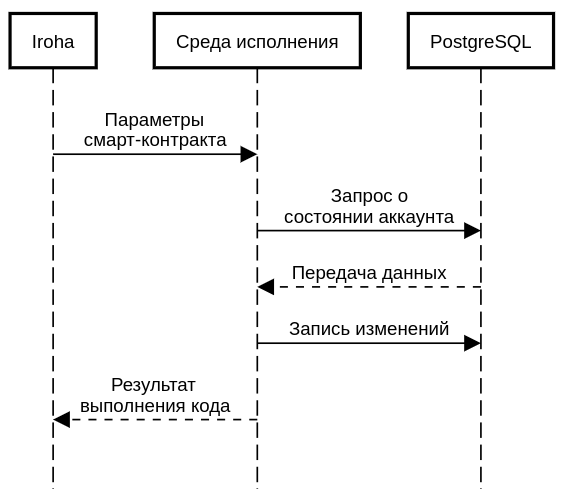
\includegraphics[scale=0.44]{inter.png}
\end{figure}
\end{frame} 

\begin{frame}{Необходимая функциональность для интеграции}
\begin{itemize}
\item Передача параметров по сети
\vfill
\item Чтение и запись актуального состояния через базу данных
\vfill
\item Формирование данных на входе и выходе в соответствии с форматом среды исполнения
\end{itemize}
\end{frame} 

\begin{frame}{Обзор существующих сред исполнения и языков смарт-контрактов}
Известные — Ethereum (Solidity, Viper), Bitcoin. Параметры сравнения: парадигма, Тьюринг-полнота, экосистема и другие.
\vfill
Обзорная статья \emph{A Survey of Smart Contract Safety and Programming Languages} для публикации в Трудах ИСП РАН.
\vfill
Ethereum --- самая развитая платформа.
\end{frame} 

\begin{frame}{Среда исполнения}
\begin{block}{Hyperledger Burrow}
Реализация блокчейна со смарт-контрактами из Ethereum ({\color{blue}{https://github.com/hyperledger/burrow}}).
\end{block}
\vfill
\begin{block}{Преимущества}
\begin{itemize}
\item Интерфейс для работы с Ethereum Virtual Machine
\vfill
\item Поддерживается сообществом Hyperledger
\vfill
\item Есть примеры интегрирования (Hyperledger Fabric и Hyperledger Seth)
\end{itemize}
\end{block}
\vfill
\begin{block}{Недостатки}
\begin{itemize}
\item Специфичная предметная область 
\end{itemize}
\end{block}

\end{frame} 

\begin{frame}{Тестирование}
\begin{block}{Команда управления}
\begin{itemize}
\item Валидация данных
\vfill
\item Операции по переводу в другой формат
\end{itemize}
\end{block}
\vfill
\begin{block}{Взаимодействие со средой исполнения}
\begin{itemize}
\item Запись
\vfill
\item Чтение
\vfill
\item Вызов функции с параметрами
\end{itemize}
\end{block}
\end{frame} 

\begin{frame}{Результаты}
\begin{itemize}
\item Выполнен обзор существующих сред исполнения и языков смарт-контрактов, обзорная статья принята для публикации в сборнике трудов ИСП РАН
\vfill
\item Разработаны архитектура и программный интерфейс для взаимодействия среды исполнения смарт-контрактов с Hyperledger Iroha
\vfill
\item Реализовано взаимодействие Hyperledger Iroha и среды исполнения смарт-контрактов проекта Hyperledger Burrow
\vfill
\item Проведено модульное и интеграционное тестирование
\end{itemize}
\end{frame} 

\begin{frame}{Использованные технологии}
\begin{block}{Языки}
	C++, Go, Solidity
\end{block}
\vfill
\begin{block}{Библиотеки}
	Libpq, GTest, Boost, Protobuf, RapidJSON
\end{block}
\vfill
\begin{block}{Дополнительно}
	PostgreSQL, EVM, CMake, Git, Docker
\end{block}

\end{frame} 

\end{document}
